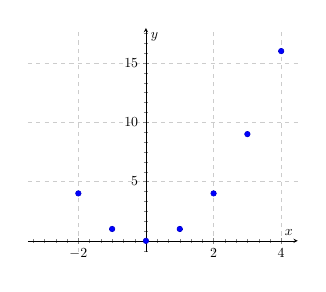
\begin{tikzpicture}[thick,scale=0.5, every node/.style={transform shape}]
  \begin{axis}[
    xmin = -3, xmax = 4, ymin = 1, ymax = 16,
    domain = -3:4,
    restrict y to domain=0:16,
    grid = major,   % both
    grid style={line width=.1pt, draw=gray!20},
    major grid style={dashed, line width=.2pt, draw=gray!40},
    minor tick num=5,
    clip = true,
    clip mode=individual,
    axis x line = middle,
    axis y line = middle,
    xlabel={$x$},
  %  xlabel style={at=(current axis.right of origin), anchor=west},
    ylabel={$y$},
  %  ylabel style={at=(current axis.above origin), anchor=south},
    enlarge y limits={rel=0.13},
    enlarge x limits={rel=0.07},
  ]
  
      \addplot[scatter, only marks, scatter src=\thisrow{class},
            error bars/.cd, 
            y dir=both, x dir=both, 
            y explicit, x explicit, 
            error bar style={color=mapped color}]
            table[x=x,y=y,x error=xerr,y error=yerr] {
                  x       xerr    y        yerr       class
                  -2.0    0.0031  4.0        0.0001   0
                  -1.0    0.0044  1.0        0.0025   0
                   0.0    0.0032  0.0        0.0012   0
                   1.0    0.0078  1.0        0.0016   0
                   2.0    0.0047  4.0        0.0002   0
                   3.0    0.0064  9.0        0.0028   0
                   4.0    0.0063 16.0        0.0004   0
      };  
  \end{axis}
\end{tikzpicture}